\section{Gold-PVD}
\label{goldpvd}

Als Testsystem für PVD-Prozesse bietet sich Gold-PVD an, die zwar durch Oberflächendiffusion dominiert wird, jedoch ideale fcc-kristalline Strukturen bildet.
Die genutzte EAM-Potentialdatei stammt aus dem \todo{ref}LAMMPS-Paket, basiert aber auf Parametern von Foiles et al.\cite{foiles_embedded-atom-method_1986}, die für Einbettung einzelner Atome in Bulk- und Oberflächensysteme optimiert wurden.

\subsection{Voruntersuchungen}

Zur Validierung grundlegender Materialeigenschaften wurden Bindungslängen, Dichten und Koordinationszahlen aus einer relaxierten kristallinen Phase untersucht (Tabelle \ref{tab:goldpreresults}).
Zur Bestimmung dieser Werte wurde ein Goldkristall von \SI{40x40x40}{\angstrom} Größe auf \SI{1000}{\kelvin} aufgeheizt, im kanonischen Ensemble relaxiert und anschließend abgekühlt.
Wie man den Ergebnissen ansehen kann, bleibt die Kristallstruktur erwartungsgemäß erhalten (die Schmelztemperatur wurde für die Relaxierung nicht überschritten) und steht in guter Übereinstimmung mit Literaturwerten.
Die Parametrisierung repräsentiert somit das Zielsystem.

\begin{table}[hbtp]
  %% \rowcolors{0}{white}{lightgray} 
  \caption[Eigenschaften von Gold]{Vergleich der Eigenschaften von Gold mit experimentellen und Literaturdaten als Voruntersuchung des PVD-Prozesses\todo[inline]{ref}}
  \label{tab:goldpreresults}
  \begin{tabularx}{\textwidth}{|lXXXX|}
    \hline
    \textbf{unters. Größe} & \textbf{Temperatur} & \textbf{Simulation} & \textbf{Experiment} & \textbf{Abweichung}\\
    \hline
    Bindungslänge  &  \SI{50}{\kelvin}   &  \SI{2.885}{\angstrom}                    &  \SI{2.884}{\angstrom}                    &  \SI{0.05}{\percent}  \\
    Koordination   &  \SI{50}{\kelvin}   &  \SI{12.00}{}                             &  \SI{12.00}{}                             &  \SI{0}{\percent}     \\
    Dichte         &  \SI{300}{\kelvin}  &  \SI{18.99}{\gram\per\cubic\centi\meter}  &  \SI{19.30}{\gram\per\cubic\centi\meter}  &  \SI{1.6}{\percent}   \\
    Dichte         &  \SI{500}{\kelvin}  &  \SI{18.89}{\gram\per\cubic\centi\meter}  &  \SI{19.13}{\gram\per\cubic\centi\meter}  &  \SI{1.2}{\percent}   \\
    \hline
  \end{tabularx}
\end{table}

\todo[inline]{Oberflächenvalidierung}

\subsection{Thermische Eigenschaften}

Neben strukturellen Eigenschaften bilden EAM-Potentiale auch einige thermische Eigenschaften von Metallen ab.
Für deren Untersuchung wurde die Massendichte in Abhängigkeit der Temperatur für die Teststruktur aufgenommen, die langsam auf \SI{2000}{\kelvin}, also weit über den Schmelzpunkt von \SI{1337}{\kelvin}, aufgeheizt wurde.
Die Ergebnisse (Abbildung \ref{fig:goldthermo}) zeigen gute Übereinstimmung mit experimentellen Daten, allerdings sind die Relaxationszeiten $t_\text{relax}$ oberhalb von ca. \SI{20}{\pico\second} und Thermostat-Dämpfungsparameter $D_T$ um \SI{0.02}{\femto\second} notwendig.

\begin{figure}[tbp]
  \centering
  \captionsetup[subfigure]{singlelinecheck=false}
  \def\subfigwidth{7cm}
  \begin{subfigure}[t]{\subfigwidth}
    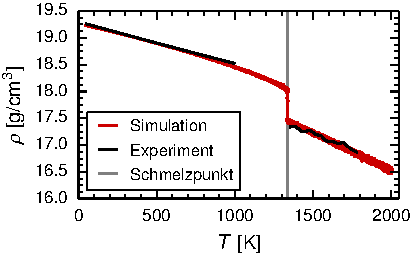
\includegraphics[width=\textwidth]{gold_bestthermo}
    \subcaption{Temperaturverlauf bei $ t_\text{relax}=\SI{50}{\pico\second}$ und $D_T=\SI{0.02}{\femto\second}$}
  \end{subfigure}
  \hfill
  \begin{subfigure}[t]{\subfigwidth}
    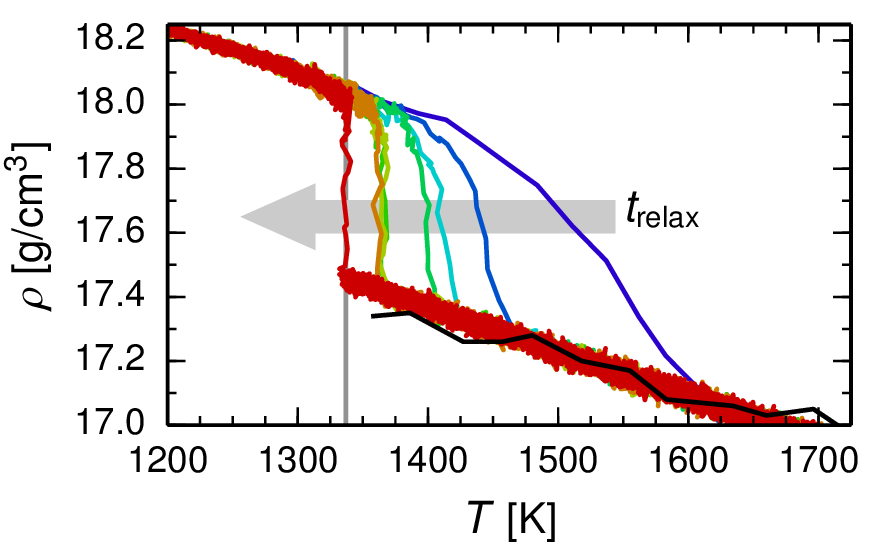
\includegraphics[width=\textwidth]{gold_relaxtime}
    \subcaption{Abhängigkeit des simulierten Schmelzpunktes von der Relaxationszeit}
  \end{subfigure}
  \caption[Ergebnisse thermischer Simulationen von Gold]{Ergebnisse thermischer Simulationen von Gold.
    Verlauf stimmt gut mit experimentellen Daten (schwarze Linien) überein.
    Experimentelle Werte stammen von aus Standardliteratur sowie von Brillo et al.\cite{brillo_density_2006}.
  }
  \label{fig:goldthermo}
\end{figure}

\subsection{Prozess-Simulation}

Zur Simulation eines Gold-PVD-Prozesses mit Parsivald wurden die untersuchten Potentialparameter sowie ein Kristallsubstrat eingelesen, ein Abscheidungsmodus mit zufälligen Auftreffpositionen in der xy-Ebene gewählt und Relaxationszeiten und Reaktionsnachbarschaftsgrößen gewählt, die in den vorheringen Tests als hinreichend ermittelt wurden.
Damit ergaben sich Reaktionsräume der Größe \SI{37x37x25}{\angstrom} mit jeweils ca. 1800 Atomen, Relaxationszeiten von \SI{1.4}{\nano\second} in \SI{1400}{} Simulationsschritten und Auftreffgeschwindigkeiten von \SI{4}{\angstrom/\pico\second}, die aus üblichen Sputterbedingungen stammen.\todo{wie berechnet?}
Die \SI{100x100}{\angstrom} breiten Kristalle werden perfekt fortgesetzt, wobei nach 10 Kristallschichten eine Rauheit von einem Atomdurchmesser vorliegt, was Übereinstimmung mit einem diffusionsdominierten Abscheidungsprozess zeigt.

\subsubsection{Strukturierte Substrate}

Als Stabilitätsprüfung wurden auch Abscheidungen auf strukturierten Substraten (Abbildung \ref{fig:goldsubstrate}) mit den gleichbleibenden Prozessbedingungen simuliert.
Es wurden Stufen und Spitzen mit Neigungen von jeweils \SI{15}{\degree}, \SI{20}{\degree}, \SI{30}{\degree}, \SI{45}{\degree}, \SI{60}{\degree} und \SI{90}{\degree} bei oben genannten Prozessbedingungen untersucht.
\todo{vorherige Relaxation?}

\begin{figure}[bt]
  \captionsetup[subfigure]{singlelinecheck=false}
  \def\subfigwidth{0.31\textwidth}
  \begin{subfigure}[t]{\subfigwidth}
    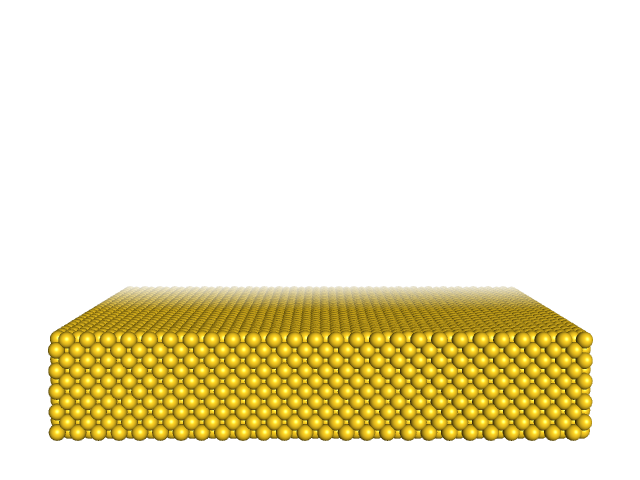
\includegraphics[width=\textwidth]{Au_substrate_flat}
    \subcaption{Glattes Gold-Substrat}
    \label{fig:goldsubstrate-a}
  \end{subfigure}
  \hfill
  \begin{subfigure}[t]{\subfigwidth}
    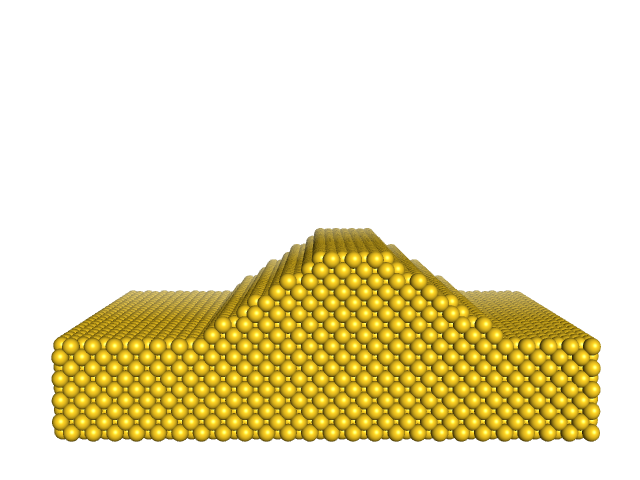
\includegraphics[width=\textwidth]{Au_substrate_step30}
    \subcaption{Gold-Stufe, \SI{30}{\degree}}
    \label{fig:goldsubstrate-b}
  \end{subfigure}
  \hfill
  \begin{subfigure}[t]{\subfigwidth}
    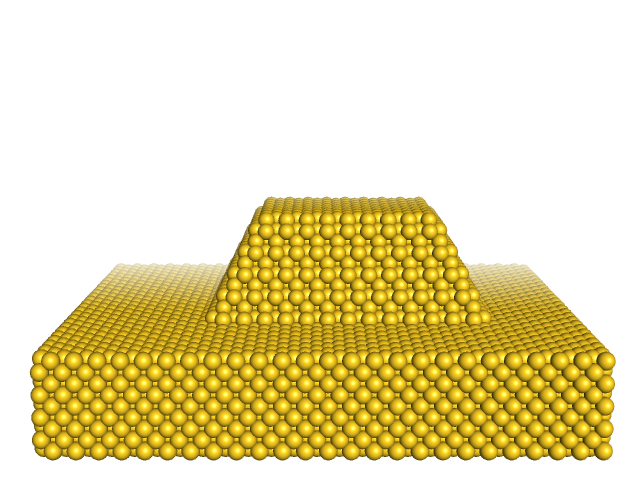
\includegraphics[width=\textwidth]{Au_substrate_tip60}
    \subcaption{Gold-Spitze, \SI{60}{\degree}}
    \label{fig:goldsubstrate-c}
  \end{subfigure}
  \caption[Strukturierte Goldsubstrate]{Goldsubstrate mit unterschiedlicher Struktur und Breite und Tiefe von \SI{100}{\angstrom}.
    Abscheidungen wurden auf glatten Substraten, Stufen und Spitzen vorgenommen.}
  \label{fig:goldsubstrate}
\end{figure}

\begin{figure}[bt]
  \captionsetup[subfigure]{singlelinecheck=false}
  \def\subfigwidth{0.31\textwidth}
  \begin{subfigure}[t]{\subfigwidth}
    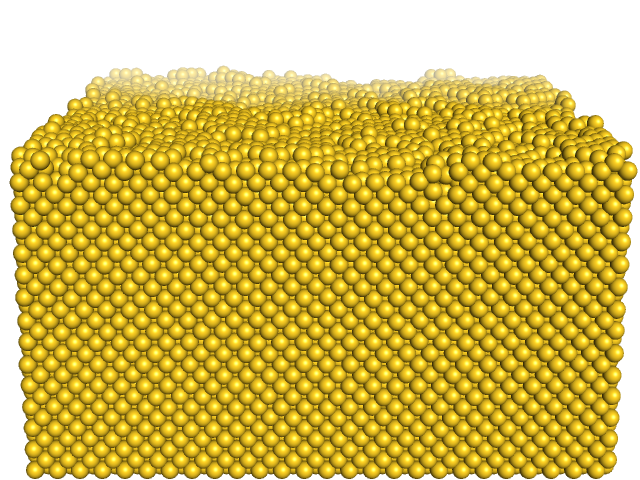
\includegraphics[width=\textwidth]{Au_deposition_flat}
    \subcaption{Abscheidung auf glattem Gold-Substrat}
    \label{fig:golddepositions-a}
  \end{subfigure}
  \hfill
  \begin{subfigure}[t]{\subfigwidth}
    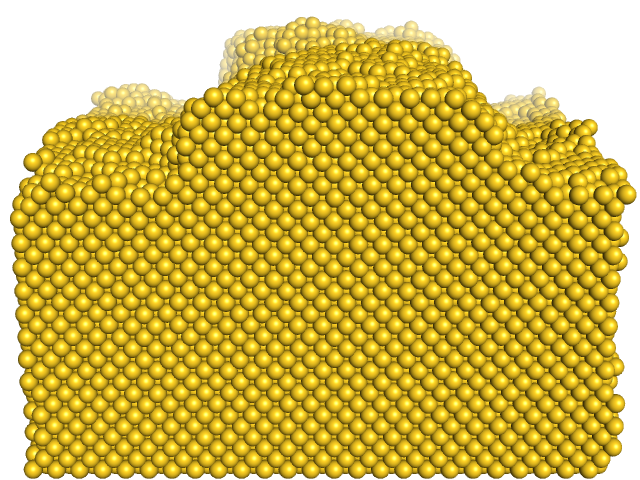
\includegraphics[width=\textwidth]{Au_deposition_step30}
    \subcaption{Abscheidung auf Gold-Stufe, \SI{30}{\degree}}
    \label{fig:golddepositions-b}
  \end{subfigure}
  \hfill
  \begin{subfigure}[t]{\subfigwidth}
    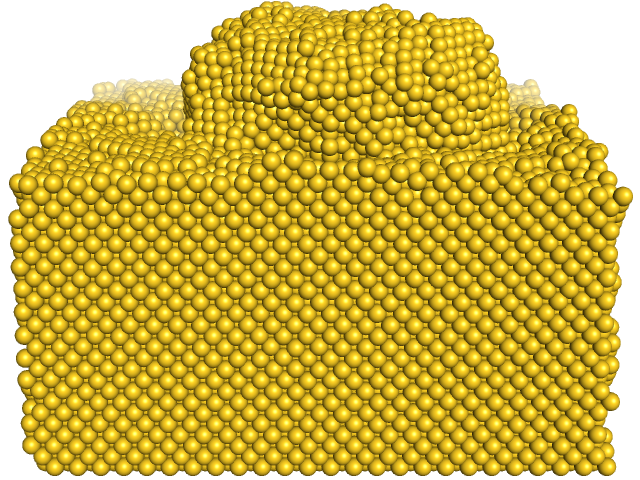
\includegraphics[width=\textwidth]{Au_deposition_tip60}
    \subcaption{Abscheidung auf Gold-Spitze, \SI{60}{\degree}}
    \label{fig:golddepositions-c}
  \end{subfigure}
  \caption[Abscheidung auf strukturierten Substraten]{
    Ergebnis der Abscheidung.
    Die Substratstruktur bleibt erkennbar, wird aber nach oben verstärkt, ansonsten aber kristallin und glatt fortgesetzt.
  }
  \label{fig:golddepositions}
\end{figure}

Das Kristallsubstrat wird auch hier fortgesetzt, jedoch verstärken sich Neigungswinkel an Stufen und Spitzen zunehmend.
Nach längeren Laufzeiten entstehen somit Überhänge, die durch Abschluss von unten zu Hohlräumen innerhalb der Struktur führen, welche in der Realität durch thermische Relaxation geschlossen würden.
Dahinter steht einerseits die Notwendigkeit, Gold-Atome bei Ankunft auf der Oberfläche ausreichend diffundieren zu lassen, was beim aktuellen Modell nur innerhalb der Reaktionsraumgrenzen geschieht.

Andererseits liegt ein methodischer Fehler bei Nutzung von Binning-Methoden vor:
Die Oberfläche wird aus algorithmischen Gründen nur entlang der z-Achse bestimmt, woraufhin das neue Atom oberhalb eines Referenzatomes auf der Oberfläche platziert wird.
An Stufen und Kanten werden hierbei höhere Reaktionsorte bevorzugt, an denen das Atom mit \todo{phrasing}statistischer Wahrscheinlichkeit verbleibt.

Einen Lösungsansatz stellt die ausführliche Parametrisierung der Oberfläche dar, beispielsweise per Alpha-Form (siehe Abschnitt \ref{dataalphaform}, über die man die Ereigniswahrscheinlichkeit entsprechend der Einbettungsenergie variierte, angenähert über die Oberflächenkrümmung.
